\documentclass[twoside]{book}

% Packages required by doxygen
\usepackage{fixltx2e}
\usepackage{calc}
\usepackage{doxygen}
\usepackage[export]{adjustbox} % also loads graphicx
\usepackage{graphicx}
\usepackage[utf8]{inputenc}
\usepackage{makeidx}
\usepackage{multicol}
\usepackage{multirow}
\PassOptionsToPackage{warn}{textcomp}
\usepackage{textcomp}
\usepackage[nointegrals]{wasysym}
\usepackage[table]{xcolor}

% Font selection
\usepackage[T1]{fontenc}
\usepackage[scaled=.90]{helvet}
\usepackage{courier}
\usepackage{amssymb}
\usepackage{sectsty}
\renewcommand{\familydefault}{\sfdefault}
\allsectionsfont{%
  \fontseries{bc}\selectfont%
  \color{darkgray}%
}
\renewcommand{\DoxyLabelFont}{%
  \fontseries{bc}\selectfont%
  \color{darkgray}%
}
\newcommand{\+}{\discretionary{\mbox{\scriptsize$\hookleftarrow$}}{}{}}

% Page & text layout
\usepackage{geometry}
\geometry{%
  a4paper,%
  top=2.5cm,%
  bottom=2.5cm,%
  left=2.5cm,%
  right=2.5cm%
}
\tolerance=750
\hfuzz=15pt
\hbadness=750
\setlength{\emergencystretch}{15pt}
\setlength{\parindent}{0cm}
\setlength{\parskip}{3ex plus 2ex minus 2ex}
\makeatletter
\renewcommand{\paragraph}{%
  \@startsection{paragraph}{4}{0ex}{-1.0ex}{1.0ex}{%
    \normalfont\normalsize\bfseries\SS@parafont%
  }%
}
\renewcommand{\subparagraph}{%
  \@startsection{subparagraph}{5}{0ex}{-1.0ex}{1.0ex}{%
    \normalfont\normalsize\bfseries\SS@subparafont%
  }%
}
\makeatother

% Headers & footers
\usepackage{fancyhdr}
\pagestyle{fancyplain}
\fancyhead[LE]{\fancyplain{}{\bfseries\thepage}}
\fancyhead[CE]{\fancyplain{}{}}
\fancyhead[RE]{\fancyplain{}{\bfseries\leftmark}}
\fancyhead[LO]{\fancyplain{}{\bfseries\rightmark}}
\fancyhead[CO]{\fancyplain{}{}}
\fancyhead[RO]{\fancyplain{}{\bfseries\thepage}}
\fancyfoot[LE]{\fancyplain{}{}}
\fancyfoot[CE]{\fancyplain{}{}}
\fancyfoot[RE]{\fancyplain{}{\bfseries\scriptsize Generated by Doxygen }}
\fancyfoot[LO]{\fancyplain{}{\bfseries\scriptsize Generated by Doxygen }}
\fancyfoot[CO]{\fancyplain{}{}}
\fancyfoot[RO]{\fancyplain{}{}}
\renewcommand{\footrulewidth}{0.4pt}
\renewcommand{\chaptermark}[1]{%
  \markboth{#1}{}%
}
\renewcommand{\sectionmark}[1]{%
  \markright{\thesection\ #1}%
}

% Indices & bibliography
\usepackage{natbib}
\usepackage[titles]{tocloft}
\setcounter{tocdepth}{3}
\setcounter{secnumdepth}{5}
\makeindex

% Hyperlinks (required, but should be loaded last)
\usepackage{ifpdf}
\ifpdf
  \usepackage[pdftex,pagebackref=true]{hyperref}
\else
  \usepackage[ps2pdf,pagebackref=true]{hyperref}
\fi
\hypersetup{%
  colorlinks=true,%
  linkcolor=blue,%
  citecolor=blue,%
  unicode%
}

% Custom commands
\newcommand{\clearemptydoublepage}{%
  \newpage{\pagestyle{empty}\cleardoublepage}%
}

\usepackage{caption}
\captionsetup{labelsep=space,justification=centering,font={bf},singlelinecheck=off,skip=4pt,position=top}

%===== C O N T E N T S =====

\begin{document}

% Titlepage & ToC
\hypersetup{pageanchor=false,
             bookmarksnumbered=true,
             pdfencoding=unicode
            }
\pagenumbering{alph}
\begin{titlepage}
\vspace*{7cm}
\begin{center}%
{\Large 2ª Projeto -\/ Tratamento de Classes Abstratas }\\
\vspace*{1cm}
{\large Generated by Doxygen 1.8.14}\\
\end{center}
\end{titlepage}
\clearemptydoublepage
\pagenumbering{roman}
\tableofcontents
\clearemptydoublepage
\pagenumbering{arabic}
\hypersetup{pageanchor=true}

%--- Begin generated contents ---
\chapter{Hierarchical Index}
\section{Class Hierarchy}
This inheritance list is sorted roughly, but not completely, alphabetically\+:\begin{DoxyCompactList}
\item \contentsline{section}{Screen}{\pageref{class_screen}}{}
\begin{DoxyCompactList}
\item \contentsline{section}{Figura\+Geometrica}{\pageref{class_figura_geometrica}}{}
\end{DoxyCompactList}
\end{DoxyCompactList}

\chapter{Class Index}
\section{Class List}
Here are the classes, structs, unions and interfaces with brief descriptions\+:\begin{DoxyCompactList}
\item\contentsline{section}{\mbox{\hyperlink{class_screen}{Screen}} \\*Para desenho em uma tela virtual }{\pageref{class_screen}}{}
\end{DoxyCompactList}

\chapter{File Index}
\section{File List}
Here is a list of all files with brief descriptions\+:\begin{DoxyCompactList}
\item\contentsline{section}{\mbox{\hyperlink{figurageometrica_8cpp}{figurageometrica.\+cpp}} }{\pageref{figurageometrica_8cpp}}{}
\item\contentsline{section}{\mbox{\hyperlink{figurageometrica_8h}{figurageometrica.\+h}} }{\pageref{figurageometrica_8h}}{}
\item\contentsline{section}{\mbox{\hyperlink{main_8cpp}{main.\+cpp}} }{\pageref{main_8cpp}}{}
\item\contentsline{section}{\mbox{\hyperlink{screen_8cpp}{screen.\+cpp}} }{\pageref{screen_8cpp}}{}
\item\contentsline{section}{\mbox{\hyperlink{screen_8h}{screen.\+h}} }{\pageref{screen_8h}}{}
\end{DoxyCompactList}

\chapter{Class Documentation}
\hypertarget{class_circulo}{}\section{Circulo Class Reference}
\label{class_circulo}\index{Circulo@{Circulo}}


The \mbox{\hyperlink{class_circulo}{Circulo}} class sera para desenhar circulos.  




{\ttfamily \#include $<$circulo.\+h$>$}

Inheritance diagram for Circulo\+:\begin{figure}[H]
\begin{center}
\leavevmode
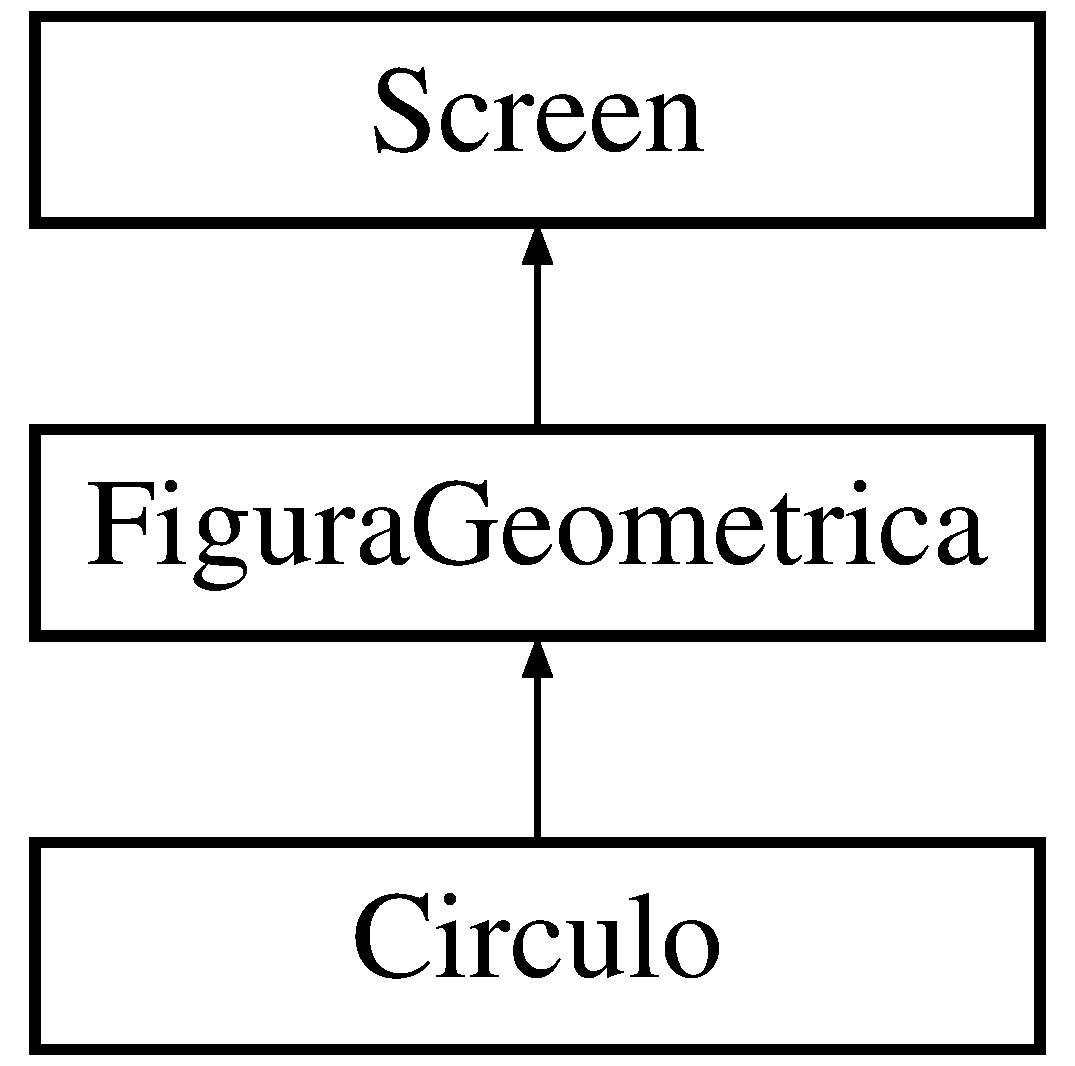
\includegraphics[height=3.000000cm]{class_circulo}
\end{center}
\end{figure}
\subsection*{Public Member Functions}
\begin{DoxyCompactItemize}
\item 
\mbox{\hyperlink{class_circulo_adbc97608526f737c01fd5f0e1fdd515b}{Circulo}} (int \+\_\+x0=0, int \+\_\+y0=0, int \+\_\+r=0, int \+\_\+f=0)
\begin{DoxyCompactList}\small\item\em \mbox{\hyperlink{class_circulo}{Circulo}} Contrutor da Class Circulos. \end{DoxyCompactList}\item 
void \mbox{\hyperlink{class_circulo_a593787d6e0618c2eded23e8839e7bea6}{draw}} (\mbox{\hyperlink{class_screen}{Screen}} \&t)
\begin{DoxyCompactList}\small\item\em draw Função que sera para desenhar o circulo. \end{DoxyCompactList}\item 
void \mbox{\hyperlink{class_circulo_a883509c096bf9c9332d749d749168c19}{pontos\+Da\+Circunferencia}} (int x, int y, \mbox{\hyperlink{class_screen}{Screen}} \&t)
\begin{DoxyCompactList}\small\item\em pontos\+Da\+Circunferencia Função pega os ponto da circunferencia. \end{DoxyCompactList}\end{DoxyCompactItemize}


\subsection{Detailed Description}
The \mbox{\hyperlink{class_circulo}{Circulo}} class sera para desenhar circulos. 

\subsection{Constructor \& Destructor Documentation}
\mbox{\Hypertarget{class_circulo_adbc97608526f737c01fd5f0e1fdd515b}\label{class_circulo_adbc97608526f737c01fd5f0e1fdd515b}} 
\index{Circulo@{Circulo}!Circulo@{Circulo}}
\index{Circulo@{Circulo}!Circulo@{Circulo}}
\subsubsection{\texorpdfstring{Circulo()}{Circulo()}}
{\footnotesize\ttfamily Circulo\+::\+Circulo (\begin{DoxyParamCaption}\item[{int}]{\+\_\+x0 = {\ttfamily 0},  }\item[{int}]{\+\_\+y0 = {\ttfamily 0},  }\item[{int}]{\+\_\+r = {\ttfamily 0},  }\item[{int}]{\+\_\+f = {\ttfamily 0} }\end{DoxyParamCaption})}



\mbox{\hyperlink{class_circulo}{Circulo}} Contrutor da Class Circulos. 


\begin{DoxyParams}{Parameters}
{\em \+\_\+x0} & paramentro X do ponto central do circulo \\
\hline
{\em \+\_\+y0} & paramentro y do ponto central do circulo \\
\hline
{\em \+\_\+r} & paramentro do raio da circulo \\
\hline
{\em \+\_\+f} & paramentro do fillmode do circulo \\
\hline
\end{DoxyParams}


\subsection{Member Function Documentation}
\mbox{\Hypertarget{class_circulo_a593787d6e0618c2eded23e8839e7bea6}\label{class_circulo_a593787d6e0618c2eded23e8839e7bea6}} 
\index{Circulo@{Circulo}!draw@{draw}}
\index{draw@{draw}!Circulo@{Circulo}}
\subsubsection{\texorpdfstring{draw()}{draw()}}
{\footnotesize\ttfamily void Circulo\+::draw (\begin{DoxyParamCaption}\item[{\mbox{\hyperlink{class_screen}{Screen}} \&}]{t }\end{DoxyParamCaption})\hspace{0.3cm}{\ttfamily [virtual]}}



draw Função que sera para desenhar o circulo. 


\begin{DoxyParams}{Parameters}
{\em t} & Tela q sera desenhado o circulo. \\
\hline
\end{DoxyParams}


Implements \mbox{\hyperlink{class_figura_geometrica_a8ee8dedc060b6059a805ea091aef2c41}{Figura\+Geometrica}}.

\mbox{\Hypertarget{class_circulo_a883509c096bf9c9332d749d749168c19}\label{class_circulo_a883509c096bf9c9332d749d749168c19}} 
\index{Circulo@{Circulo}!pontos\+Da\+Circunferencia@{pontos\+Da\+Circunferencia}}
\index{pontos\+Da\+Circunferencia@{pontos\+Da\+Circunferencia}!Circulo@{Circulo}}
\subsubsection{\texorpdfstring{pontos\+Da\+Circunferencia()}{pontosDaCircunferencia()}}
{\footnotesize\ttfamily void Circulo\+::pontos\+Da\+Circunferencia (\begin{DoxyParamCaption}\item[{int}]{x,  }\item[{int}]{y,  }\item[{\mbox{\hyperlink{class_screen}{Screen}} \&}]{t }\end{DoxyParamCaption})}



pontos\+Da\+Circunferencia Função pega os ponto da circunferencia. 


\begin{DoxyParams}{Parameters}
{\em x} & paramentro da coordenada x usando para o calculo. \\
\hline
{\em y} & parametro da coordenada y usado para o calculo. \\
\hline
{\em t} & Tela que será usado para os calculos. \\
\hline
\end{DoxyParams}


The documentation for this class was generated from the following files\+:\begin{DoxyCompactItemize}
\item 
\mbox{\hyperlink{circulo_8h}{circulo.\+h}}\item 
\mbox{\hyperlink{circulo_8cpp}{circulo.\+cpp}}\end{DoxyCompactItemize}

\hypertarget{class_figura_geometrica}{}\section{Figura\+Geometrica Class Reference}
\label{class_figura_geometrica}\index{Figura\+Geometrica@{Figura\+Geometrica}}


The \mbox{\hyperlink{class_figura_geometrica}{Figura\+Geometrica}} class classe abstrata \mbox{\hyperlink{class_figura_geometrica}{Figura\+Geometrica}} para representar objetos primitivos genéricos.  




{\ttfamily \#include $<$figurageometrica.\+h$>$}

Inheritance diagram for Figura\+Geometrica\+:\begin{figure}[H]
\begin{center}
\leavevmode
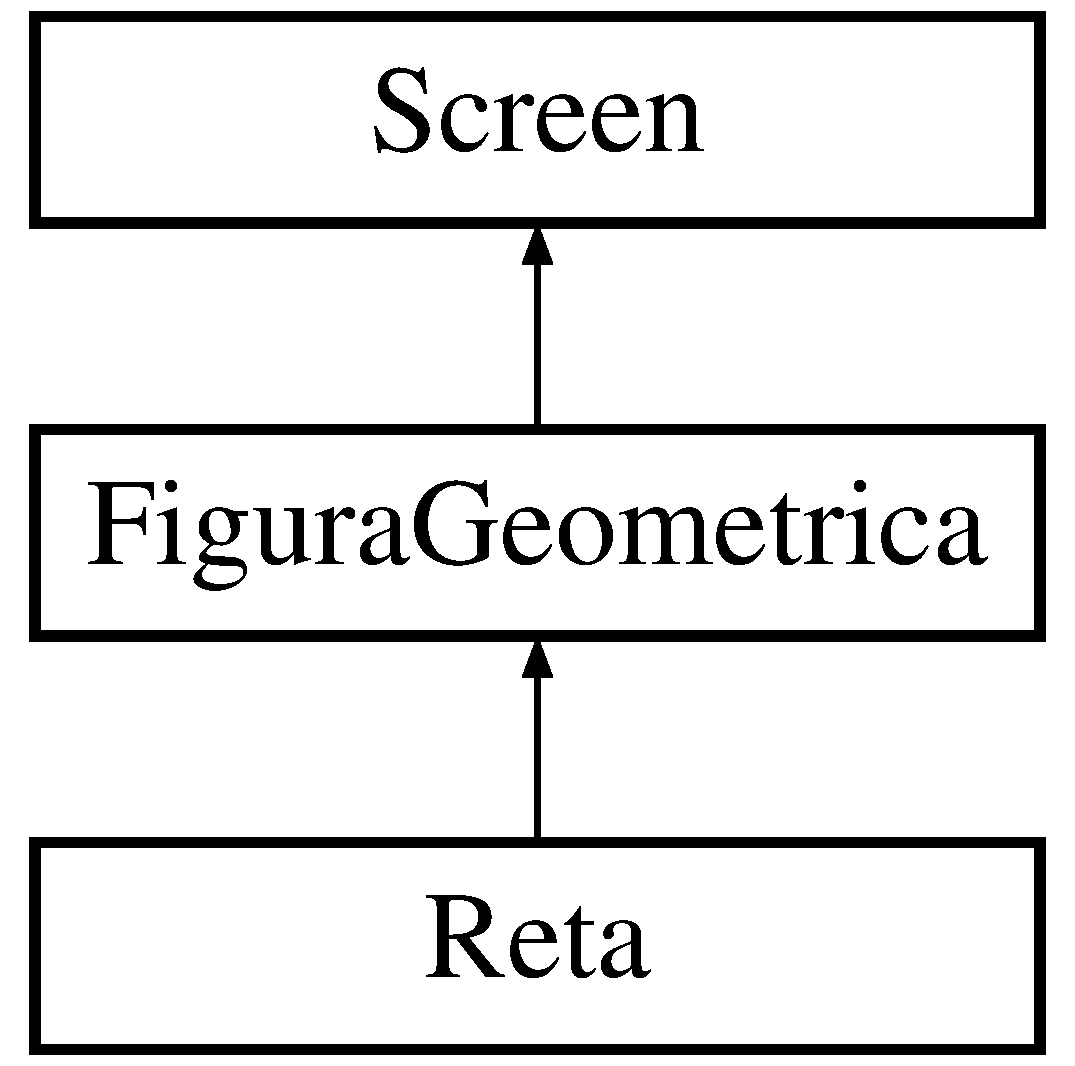
\includegraphics[height=3.000000cm]{class_figura_geometrica}
\end{center}
\end{figure}
\subsection*{Public Member Functions}
\begin{DoxyCompactItemize}
\item 
virtual void \mbox{\hyperlink{class_figura_geometrica_a8ee8dedc060b6059a805ea091aef2c41}{draw}} (\mbox{\hyperlink{class_screen}{Screen}} \&t)=0
\begin{DoxyCompactList}\small\item\em draw Uma função virtual pura que instrua o objeto a se desenhar em um objeto do tipo \mbox{\hyperlink{class_screen}{Screen}} \end{DoxyCompactList}\end{DoxyCompactItemize}


\subsection{Detailed Description}
The \mbox{\hyperlink{class_figura_geometrica}{Figura\+Geometrica}} class classe abstrata \mbox{\hyperlink{class_figura_geometrica}{Figura\+Geometrica}} para representar objetos primitivos genéricos. 

\subsection{Member Function Documentation}
\mbox{\Hypertarget{class_figura_geometrica_a8ee8dedc060b6059a805ea091aef2c41}\label{class_figura_geometrica_a8ee8dedc060b6059a805ea091aef2c41}} 
\index{Figura\+Geometrica@{Figura\+Geometrica}!draw@{draw}}
\index{draw@{draw}!Figura\+Geometrica@{Figura\+Geometrica}}
\subsubsection{\texorpdfstring{draw()}{draw()}}
{\footnotesize\ttfamily virtual void Figura\+Geometrica\+::draw (\begin{DoxyParamCaption}\item[{\mbox{\hyperlink{class_screen}{Screen}} \&}]{t }\end{DoxyParamCaption})\hspace{0.3cm}{\ttfamily [pure virtual]}}



draw Uma função virtual pura que instrua o objeto a se desenhar em um objeto do tipo \mbox{\hyperlink{class_screen}{Screen}} 


\begin{DoxyParams}{Parameters}
{\em t} & Tela no qual sera desenhado o objeto desejado \\
\hline
\end{DoxyParams}


Implemented in \mbox{\hyperlink{class_reta_ac2e9805183cd474b62bffd8b032cd780}{Reta}}.



The documentation for this class was generated from the following file\+:\begin{DoxyCompactItemize}
\item 
\mbox{\hyperlink{figurageometrica_8h}{figurageometrica.\+h}}\end{DoxyCompactItemize}

\hypertarget{class_reta}{}\section{Reta Class Reference}
\label{class_reta}\index{Reta@{Reta}}


The \mbox{\hyperlink{class_reta}{Reta}} class é uma classe derivada da classe \mbox{\hyperlink{class_figura_geometrica}{Figura\+Geometrica}}.  




{\ttfamily \#include $<$reta.\+h$>$}

Inheritance diagram for Reta\+:\begin{figure}[H]
\begin{center}
\leavevmode
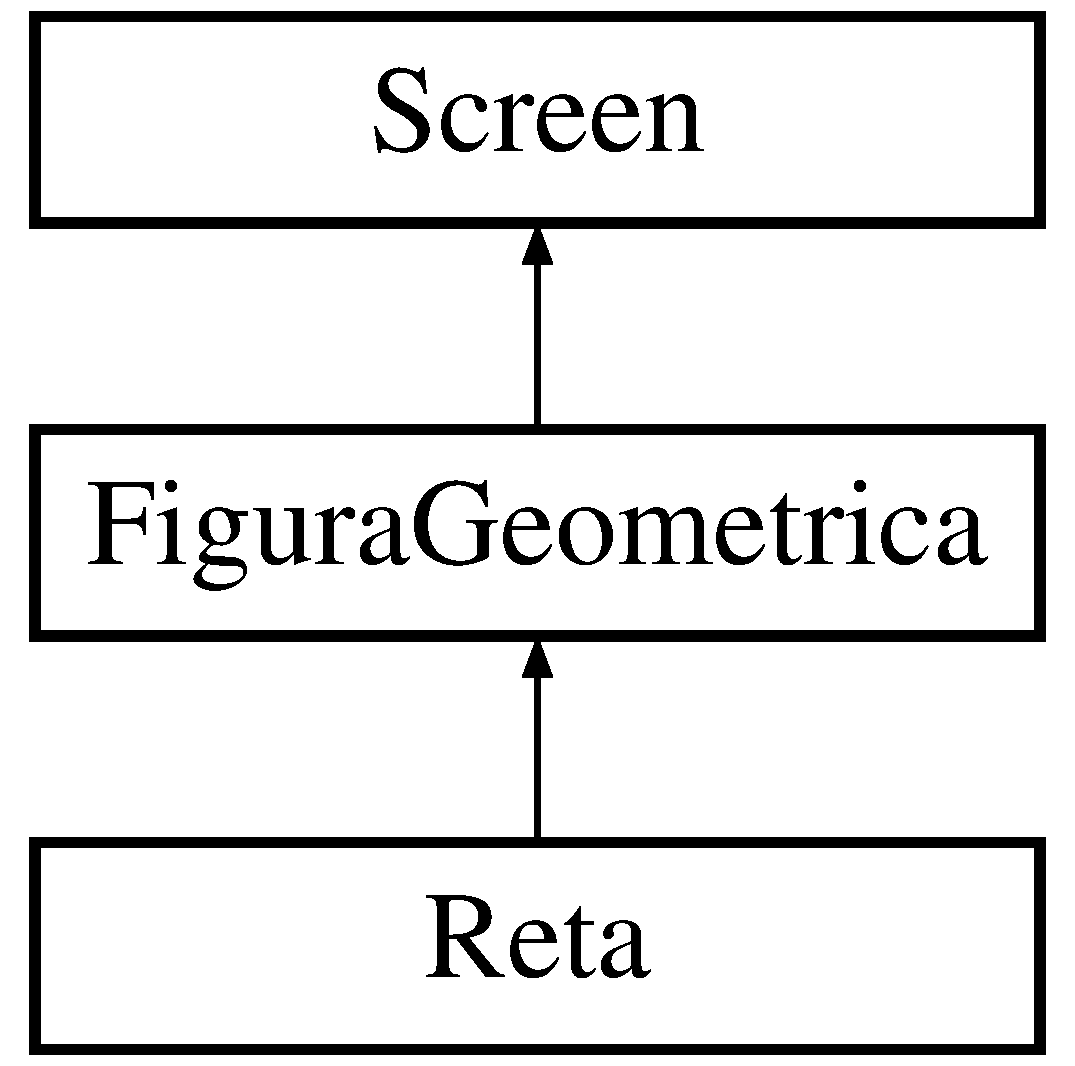
\includegraphics[height=3.000000cm]{class_reta}
\end{center}
\end{figure}
\subsection*{Public Member Functions}
\begin{DoxyCompactItemize}
\item 
\mbox{\hyperlink{class_reta_a097fd952fee835799da0f3d79b926b56}{Reta}} (int \+\_\+x0=0, int \+\_\+y0=0, int \+\_\+x1=0, int \+\_\+y1=0)
\begin{DoxyCompactList}\small\item\em \mbox{\hyperlink{class_reta}{Reta}} é o contrutor da class \mbox{\hyperlink{class_reta}{Reta}}. \end{DoxyCompactList}\item 
void \mbox{\hyperlink{class_reta_ac2e9805183cd474b62bffd8b032cd780}{draw}} (\mbox{\hyperlink{class_screen}{Screen}} \&t)
\begin{DoxyCompactList}\small\item\em draw Função que desenha uma reta na tela passado como paramentro. \end{DoxyCompactList}\end{DoxyCompactItemize}


\subsection{Detailed Description}
The \mbox{\hyperlink{class_reta}{Reta}} class é uma classe derivada da classe \mbox{\hyperlink{class_figura_geometrica}{Figura\+Geometrica}}. 

\subsection{Constructor \& Destructor Documentation}
\mbox{\Hypertarget{class_reta_a097fd952fee835799da0f3d79b926b56}\label{class_reta_a097fd952fee835799da0f3d79b926b56}} 
\index{Reta@{Reta}!Reta@{Reta}}
\index{Reta@{Reta}!Reta@{Reta}}
\subsubsection{\texorpdfstring{Reta()}{Reta()}}
{\footnotesize\ttfamily Reta\+::\+Reta (\begin{DoxyParamCaption}\item[{int}]{\+\_\+x0 = {\ttfamily 0},  }\item[{int}]{\+\_\+y0 = {\ttfamily 0},  }\item[{int}]{\+\_\+x1 = {\ttfamily 0},  }\item[{int}]{\+\_\+y1 = {\ttfamily 0} }\end{DoxyParamCaption})}



\mbox{\hyperlink{class_reta}{Reta}} é o contrutor da class \mbox{\hyperlink{class_reta}{Reta}}. 


\begin{DoxyParams}{Parameters}
{\em \+\_\+x0} & Ponto x inicial \\
\hline
{\em \+\_\+y0} & Ponto y inicial \\
\hline
{\em \+\_\+x1} & Ponto x final \\
\hline
{\em \+\_\+y1} & Ponto y final \\
\hline
\end{DoxyParams}


\subsection{Member Function Documentation}
\mbox{\Hypertarget{class_reta_ac2e9805183cd474b62bffd8b032cd780}\label{class_reta_ac2e9805183cd474b62bffd8b032cd780}} 
\index{Reta@{Reta}!draw@{draw}}
\index{draw@{draw}!Reta@{Reta}}
\subsubsection{\texorpdfstring{draw()}{draw()}}
{\footnotesize\ttfamily void Reta\+::draw (\begin{DoxyParamCaption}\item[{\mbox{\hyperlink{class_screen}{Screen}} \&}]{t }\end{DoxyParamCaption})\hspace{0.3cm}{\ttfamily [virtual]}}



draw Função que desenha uma reta na tela passado como paramentro. 


\begin{DoxyParams}{Parameters}
{\em t} & Tela que sera desenhado a \mbox{\hyperlink{class_reta}{Reta}}. \\
\hline
\end{DoxyParams}


Implements \mbox{\hyperlink{class_figura_geometrica_a8ee8dedc060b6059a805ea091aef2c41}{Figura\+Geometrica}}.



The documentation for this class was generated from the following files\+:\begin{DoxyCompactItemize}
\item 
\mbox{\hyperlink{reta_8h}{reta.\+h}}\item 
\mbox{\hyperlink{reta_8cpp}{reta.\+cpp}}\end{DoxyCompactItemize}

\hypertarget{class_retangulo}{}\section{Retangulo Class Reference}
\label{class_retangulo}\index{Retangulo@{Retangulo}}


The \mbox{\hyperlink{class_retangulo}{Retangulo}} class Serve para construir Retangulos.  




{\ttfamily \#include $<$retangulo.\+h$>$}

Inheritance diagram for Retangulo\+:\begin{figure}[H]
\begin{center}
\leavevmode
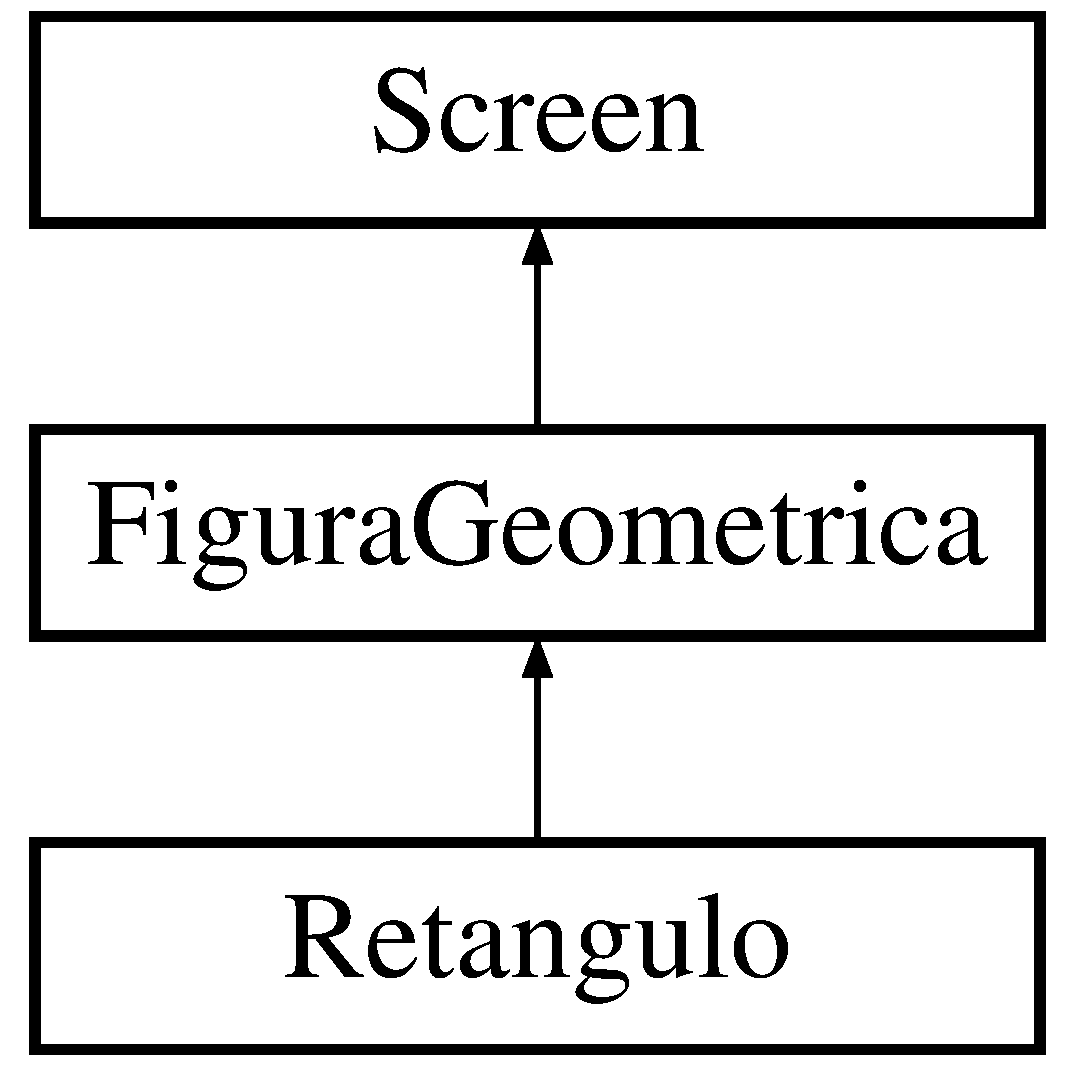
\includegraphics[height=3.000000cm]{class_retangulo}
\end{center}
\end{figure}
\subsection*{Public Member Functions}
\begin{DoxyCompactItemize}
\item 
\mbox{\hyperlink{class_retangulo_a8aa0361c5e9fb4c0df3a000858f51d8a}{Retangulo}} (int \+\_\+x0=0, int \+\_\+y0=0, int \+\_\+larg=0, int \+\_\+alt=0, int fill=0)
\begin{DoxyCompactList}\small\item\em \mbox{\hyperlink{class_retangulo}{Retangulo}} Contrutor da Class \mbox{\hyperlink{class_retangulo}{Retangulo}}. \end{DoxyCompactList}\item 
void \mbox{\hyperlink{class_retangulo_ac088dd6d3f4f3d3f80363a868c2e74f1}{draw}} (\mbox{\hyperlink{class_screen}{Screen}} \&t)
\begin{DoxyCompactList}\small\item\em draw Função que desenha na tela passada o retangulo \end{DoxyCompactList}\end{DoxyCompactItemize}


\subsection{Detailed Description}
The \mbox{\hyperlink{class_retangulo}{Retangulo}} class Serve para construir Retangulos. 

\subsection{Constructor \& Destructor Documentation}
\mbox{\Hypertarget{class_retangulo_a8aa0361c5e9fb4c0df3a000858f51d8a}\label{class_retangulo_a8aa0361c5e9fb4c0df3a000858f51d8a}} 
\index{Retangulo@{Retangulo}!Retangulo@{Retangulo}}
\index{Retangulo@{Retangulo}!Retangulo@{Retangulo}}
\subsubsection{\texorpdfstring{Retangulo()}{Retangulo()}}
{\footnotesize\ttfamily Retangulo\+::\+Retangulo (\begin{DoxyParamCaption}\item[{int}]{\+\_\+x0 = {\ttfamily 0},  }\item[{int}]{\+\_\+y0 = {\ttfamily 0},  }\item[{int}]{\+\_\+larg = {\ttfamily 0},  }\item[{int}]{\+\_\+alt = {\ttfamily 0},  }\item[{int}]{fill = {\ttfamily 0} }\end{DoxyParamCaption})}



\mbox{\hyperlink{class_retangulo}{Retangulo}} Contrutor da Class \mbox{\hyperlink{class_retangulo}{Retangulo}}. 


\begin{DoxyParams}{Parameters}
{\em \+\_\+x0} & coordenada x0 do ponto superior esquerdo do retangulo \\
\hline
{\em \+\_\+y0} & coordenada y0 do ponto superior esquerdo do retangulo \\
\hline
{\em \+\_\+larg} & paramentro para a largura do retangulo \\
\hline
{\em \+\_\+alt} & paramentro para a altura do retangulo \\
\hline
{\em fill} & paramentro para o fillmode do retangulo \\
\hline
\end{DoxyParams}


\subsection{Member Function Documentation}
\mbox{\Hypertarget{class_retangulo_ac088dd6d3f4f3d3f80363a868c2e74f1}\label{class_retangulo_ac088dd6d3f4f3d3f80363a868c2e74f1}} 
\index{Retangulo@{Retangulo}!draw@{draw}}
\index{draw@{draw}!Retangulo@{Retangulo}}
\subsubsection{\texorpdfstring{draw()}{draw()}}
{\footnotesize\ttfamily void Retangulo\+::draw (\begin{DoxyParamCaption}\item[{\mbox{\hyperlink{class_screen}{Screen}} \&}]{t }\end{DoxyParamCaption})\hspace{0.3cm}{\ttfamily [virtual]}}



draw Função que desenha na tela passada o retangulo 


\begin{DoxyParams}{Parameters}
{\em t} & Tela que será utilizada para desenho. \\
\hline
\end{DoxyParams}


Implements \mbox{\hyperlink{class_figura_geometrica_a8ee8dedc060b6059a805ea091aef2c41}{Figura\+Geometrica}}.



The documentation for this class was generated from the following files\+:\begin{DoxyCompactItemize}
\item 
\mbox{\hyperlink{retangulo_8h}{retangulo.\+h}}\item 
\mbox{\hyperlink{retangulo_8cpp}{retangulo.\+cpp}}\end{DoxyCompactItemize}

\hypertarget{class_screen}{}\section{Screen Class Reference}
\label{class_screen}\index{Screen@{Screen}}


The \mbox{\hyperlink{class_screen}{Screen}} class para desenho em uma tela virtual.  




{\ttfamily \#include $<$screen.\+h$>$}

Inheritance diagram for Screen\+:\begin{figure}[H]
\begin{center}
\leavevmode
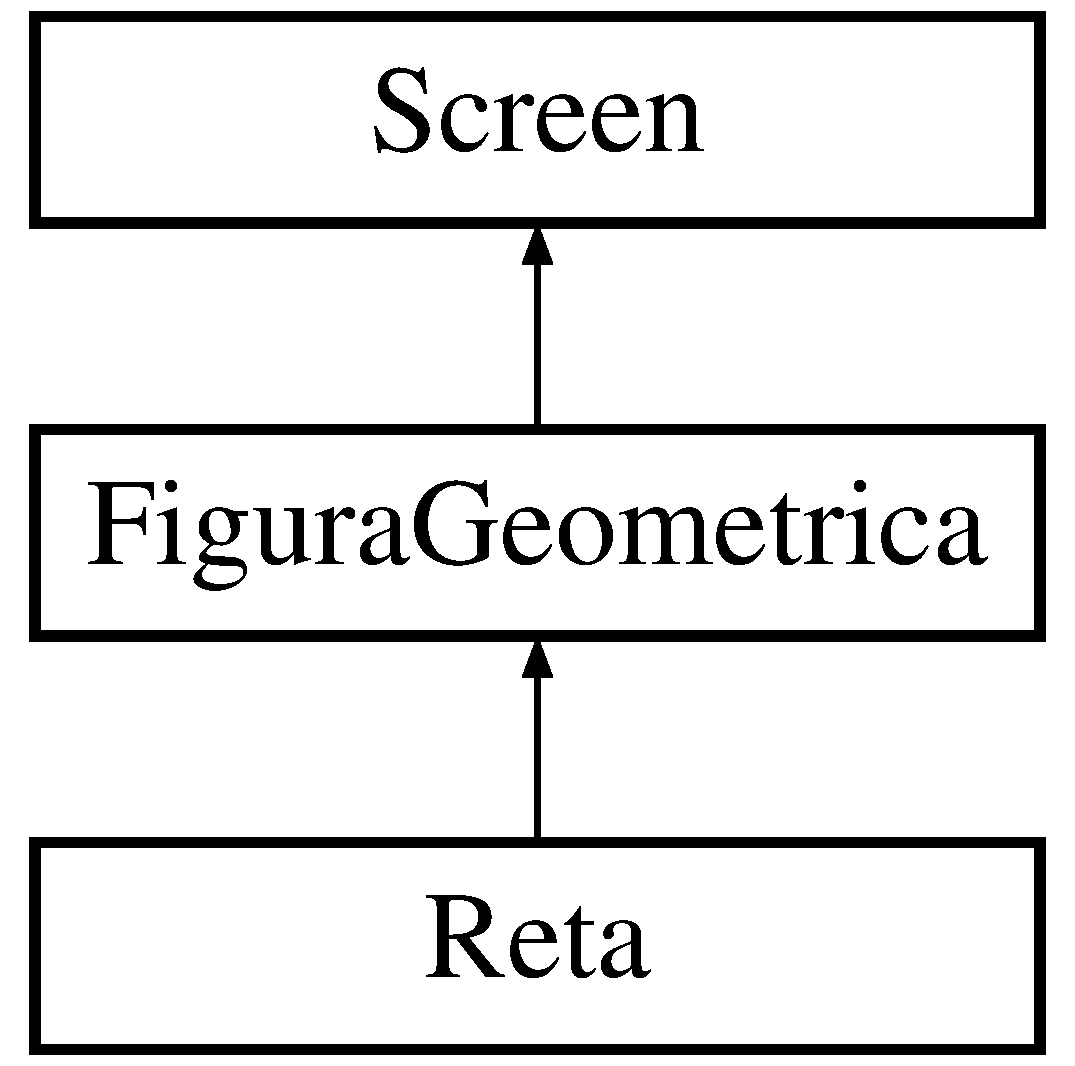
\includegraphics[height=3.000000cm]{class_screen}
\end{center}
\end{figure}
\subsection*{Public Member Functions}
\begin{DoxyCompactItemize}
\item 
\mbox{\hyperlink{class_screen_ac0cb3fd57e5eb225d9756b8eb6311833}{Screen}} (int \+\_\+nlin=0, int \+\_\+ncol=0)
\begin{DoxyCompactList}\small\item\em \mbox{\hyperlink{class_screen}{Screen}} Construtor da Class Scren. \end{DoxyCompactList}\item 
\mbox{\hyperlink{class_screen_a4243bc17596af96415b09ac48205676d}{$\sim$\+Screen}} ()
\item 
void \mbox{\hyperlink{class_screen_ae6bea81c57a22d226507c3c26fa95ee0}{set\+Pixel}} (int x, int y)
\begin{DoxyCompactList}\small\item\em set\+Pixel Função que desenha na tela; \end{DoxyCompactList}\item 
void \mbox{\hyperlink{class_screen_a35e74266b2a04e37b354ceff7a5f1031}{clear}} ()
\begin{DoxyCompactList}\small\item\em clear Função que Limpa a tela; \end{DoxyCompactList}\item 
void \mbox{\hyperlink{class_screen_aebc4eb6cb5acf15a0f04c1494622ab23}{set\+Brush}} (char \+\_\+brush)
\begin{DoxyCompactList}\small\item\em set\+Brush Função que set o pincel para desenho; \end{DoxyCompactList}\end{DoxyCompactItemize}
\subsection*{Friends}
\begin{DoxyCompactItemize}
\item 
ostream \& \mbox{\hyperlink{class_screen_aab6a2880746bfe1b7964817cc8f0989e}{operator$<$$<$}} (ostream \&os, \mbox{\hyperlink{class_screen}{Screen}} \&t)
\begin{DoxyCompactList}\small\item\em operator $<$$<$ Função que funciona como fluxo de saida; \end{DoxyCompactList}\end{DoxyCompactItemize}


\subsection{Detailed Description}
The \mbox{\hyperlink{class_screen}{Screen}} class para desenho em uma tela virtual. 

\subsection{Constructor \& Destructor Documentation}
\mbox{\Hypertarget{class_screen_ac0cb3fd57e5eb225d9756b8eb6311833}\label{class_screen_ac0cb3fd57e5eb225d9756b8eb6311833}} 
\index{Screen@{Screen}!Screen@{Screen}}
\index{Screen@{Screen}!Screen@{Screen}}
\subsubsection{\texorpdfstring{Screen()}{Screen()}}
{\footnotesize\ttfamily Screen\+::\+Screen (\begin{DoxyParamCaption}\item[{int}]{\+\_\+nlin = {\ttfamily 0},  }\item[{int}]{\+\_\+ncol = {\ttfamily 0} }\end{DoxyParamCaption})}



\mbox{\hyperlink{class_screen}{Screen}} Construtor da Class Scren. 


\begin{DoxyParams}{Parameters}
{\em nlin} & Variavel para o tamanho da linhas da Matriz. \\
\hline
{\em ncol} & Variavel para o tamanho de colunas da Matriz. \\
\hline
\end{DoxyParams}
\mbox{\Hypertarget{class_screen_a4243bc17596af96415b09ac48205676d}\label{class_screen_a4243bc17596af96415b09ac48205676d}} 
\index{Screen@{Screen}!````~Screen@{$\sim$\+Screen}}
\index{````~Screen@{$\sim$\+Screen}!Screen@{Screen}}
\subsubsection{\texorpdfstring{$\sim$\+Screen()}{~Screen()}}
{\footnotesize\ttfamily Screen\+::$\sim$\+Screen (\begin{DoxyParamCaption}{ }\end{DoxyParamCaption})}



\subsection{Member Function Documentation}
\mbox{\Hypertarget{class_screen_a35e74266b2a04e37b354ceff7a5f1031}\label{class_screen_a35e74266b2a04e37b354ceff7a5f1031}} 
\index{Screen@{Screen}!clear@{clear}}
\index{clear@{clear}!Screen@{Screen}}
\subsubsection{\texorpdfstring{clear()}{clear()}}
{\footnotesize\ttfamily void Screen\+::clear (\begin{DoxyParamCaption}{ }\end{DoxyParamCaption})}



clear Função que Limpa a tela; 

\mbox{\Hypertarget{class_screen_aebc4eb6cb5acf15a0f04c1494622ab23}\label{class_screen_aebc4eb6cb5acf15a0f04c1494622ab23}} 
\index{Screen@{Screen}!set\+Brush@{set\+Brush}}
\index{set\+Brush@{set\+Brush}!Screen@{Screen}}
\subsubsection{\texorpdfstring{set\+Brush()}{setBrush()}}
{\footnotesize\ttfamily void Screen\+::set\+Brush (\begin{DoxyParamCaption}\item[{char}]{\+\_\+brush }\end{DoxyParamCaption})}



set\+Brush Função que set o pincel para desenho; 


\begin{DoxyParams}{Parameters}
{\em \+\_\+brush} & Variavel que diz qual sera o pincel \\
\hline
\end{DoxyParams}
\mbox{\Hypertarget{class_screen_ae6bea81c57a22d226507c3c26fa95ee0}\label{class_screen_ae6bea81c57a22d226507c3c26fa95ee0}} 
\index{Screen@{Screen}!set\+Pixel@{set\+Pixel}}
\index{set\+Pixel@{set\+Pixel}!Screen@{Screen}}
\subsubsection{\texorpdfstring{set\+Pixel()}{setPixel()}}
{\footnotesize\ttfamily void Screen\+::set\+Pixel (\begin{DoxyParamCaption}\item[{int}]{x,  }\item[{int}]{y }\end{DoxyParamCaption})}



set\+Pixel Função que desenha na tela; 


\begin{DoxyParams}{Parameters}
{\em x} & posição da largura da matriz; \\
\hline
{\em y} & posição da coluna da matriz; \\
\hline
\end{DoxyParams}


\subsection{Friends And Related Function Documentation}
\mbox{\Hypertarget{class_screen_aab6a2880746bfe1b7964817cc8f0989e}\label{class_screen_aab6a2880746bfe1b7964817cc8f0989e}} 
\index{Screen@{Screen}!operator$<$$<$@{operator$<$$<$}}
\index{operator$<$$<$@{operator$<$$<$}!Screen@{Screen}}
\subsubsection{\texorpdfstring{operator$<$$<$}{operator<<}}
{\footnotesize\ttfamily ostream\& operator$<$$<$ (\begin{DoxyParamCaption}\item[{ostream \&}]{os,  }\item[{\mbox{\hyperlink{class_screen}{Screen}} \&}]{t }\end{DoxyParamCaption})\hspace{0.3cm}{\ttfamily [friend]}}



operator $<$$<$ Função que funciona como fluxo de saida; 


\begin{DoxyParams}{Parameters}
{\em os} & Variavel do fluxo de saida; \\
\hline
{\em t} & Variavel da Tela que você gostaria de mostrar \\
\hline
\end{DoxyParams}
\begin{DoxyReturn}{Returns}
Retorna o fluxo de saida 
\end{DoxyReturn}


The documentation for this class was generated from the following files\+:\begin{DoxyCompactItemize}
\item 
\mbox{\hyperlink{screen_8h}{screen.\+h}}\item 
\mbox{\hyperlink{screen_8cpp}{screen.\+cpp}}\end{DoxyCompactItemize}

\chapter{File Documentation}
\hypertarget{circulo_8cpp}{}\section{circulo.\+cpp File Reference}
\label{circulo_8cpp}\index{circulo.\+cpp@{circulo.\+cpp}}
{\ttfamily \#include \char`\"{}circulo.\+h\char`\"{}}\newline
{\ttfamily \#include $<$math.\+h$>$}\newline

\hypertarget{circulo_8h}{}\section{circulo.\+h File Reference}
\label{circulo_8h}\index{circulo.\+h@{circulo.\+h}}
{\ttfamily \#include \char`\"{}figurageometrica.\+h\char`\"{}}\newline
\subsection*{Classes}
\begin{DoxyCompactItemize}
\item 
class \mbox{\hyperlink{class_circulo}{Circulo}}
\begin{DoxyCompactList}\small\item\em The \mbox{\hyperlink{class_circulo}{Circulo}} class sera para desenhar circulos. \end{DoxyCompactList}\end{DoxyCompactItemize}

\hypertarget{figurageometrica_8h}{}\section{figurageometrica.\+h File Reference}
\label{figurageometrica_8h}\index{figurageometrica.\+h@{figurageometrica.\+h}}
\subsection*{Classes}
\begin{DoxyCompactItemize}
\item 
class \mbox{\hyperlink{class_figura_geometrica}{Figura\+Geometrica}}
\end{DoxyCompactItemize}

\hypertarget{main_8cpp}{}\section{main.\+cpp File Reference}
\label{main_8cpp}\index{main.\+cpp@{main.\+cpp}}
{\ttfamily \#include $<$iostream$>$}\newline
{\ttfamily \#include $<$vector$>$}\newline
{\ttfamily \#include \char`\"{}screen.\+h\char`\"{}}\newline
{\ttfamily \#include $<$fstream$>$}\newline
{\ttfamily \#include $<$sstream$>$}\newline
{\ttfamily \#include $<$string$>$}\newline
\subsection*{Functions}
\begin{DoxyCompactItemize}
\item 
int \mbox{\hyperlink{main_8cpp_ae66f6b31b5ad750f1fe042a706a4e3d4}{main}} ()
\end{DoxyCompactItemize}


\subsection{Function Documentation}
\mbox{\Hypertarget{main_8cpp_ae66f6b31b5ad750f1fe042a706a4e3d4}\label{main_8cpp_ae66f6b31b5ad750f1fe042a706a4e3d4}} 
\index{main.\+cpp@{main.\+cpp}!main@{main}}
\index{main@{main}!main.\+cpp@{main.\+cpp}}
\subsubsection{\texorpdfstring{main()}{main()}}
{\footnotesize\ttfamily int main (\begin{DoxyParamCaption}{ }\end{DoxyParamCaption})}


\hypertarget{reta_8cpp}{}\section{reta.\+cpp File Reference}
\label{reta_8cpp}\index{reta.\+cpp@{reta.\+cpp}}
{\ttfamily \#include \char`\"{}reta.\+h\char`\"{}}\newline
{\ttfamily \#include $<$iostream$>$}\newline
\subsection*{Functions}
\begin{DoxyCompactItemize}
\item 
int \mbox{\hyperlink{reta_8cpp_a7a68d85281d5ca5daa64fd69dfd1a981}{Sinal}} (int s)
\end{DoxyCompactItemize}


\subsection{Function Documentation}
\mbox{\Hypertarget{reta_8cpp_a7a68d85281d5ca5daa64fd69dfd1a981}\label{reta_8cpp_a7a68d85281d5ca5daa64fd69dfd1a981}} 
\index{reta.\+cpp@{reta.\+cpp}!Sinal@{Sinal}}
\index{Sinal@{Sinal}!reta.\+cpp@{reta.\+cpp}}
\subsubsection{\texorpdfstring{Sinal()}{Sinal()}}
{\footnotesize\ttfamily int Sinal (\begin{DoxyParamCaption}\item[{int}]{s }\end{DoxyParamCaption})}


\hypertarget{reta_8h}{}\section{reta.\+h File Reference}
\label{reta_8h}\index{reta.\+h@{reta.\+h}}
{\ttfamily \#include \char`\"{}figurageometrica.\+h\char`\"{}}\newline
\subsection*{Classes}
\begin{DoxyCompactItemize}
\item 
class \mbox{\hyperlink{class_reta}{Reta}}
\begin{DoxyCompactList}\small\item\em The \mbox{\hyperlink{class_reta}{Reta}} class é uma classe derivada da classe \mbox{\hyperlink{class_figura_geometrica}{Figura\+Geometrica}}. \end{DoxyCompactList}\end{DoxyCompactItemize}

\hypertarget{retangulo_8cpp}{}\section{retangulo.\+cpp File Reference}
\label{retangulo_8cpp}\index{retangulo.\+cpp@{retangulo.\+cpp}}
{\ttfamily \#include \char`\"{}retangulo.\+h\char`\"{}}\newline
{\ttfamily \#include $<$iostream$>$}\newline

\hypertarget{retangulo_8h}{}\section{retangulo.\+h File Reference}
\label{retangulo_8h}\index{retangulo.\+h@{retangulo.\+h}}
{\ttfamily \#include \char`\"{}figurageometrica.\+h\char`\"{}}\newline
\subsection*{Classes}
\begin{DoxyCompactItemize}
\item 
class \mbox{\hyperlink{class_retangulo}{Retangulo}}
\begin{DoxyCompactList}\small\item\em The \mbox{\hyperlink{class_retangulo}{Retangulo}} class Serve para construir Retangulos. \end{DoxyCompactList}\end{DoxyCompactItemize}

\hypertarget{screen_8cpp}{}\section{screen.\+cpp File Reference}
\label{screen_8cpp}\index{screen.\+cpp@{screen.\+cpp}}
{\ttfamily \#include \char`\"{}screen.\+h\char`\"{}}\newline
{\ttfamily \#include $<$iostream$>$}\newline
{\ttfamily \#include $<$vector$>$}\newline
\subsection*{Functions}
\begin{DoxyCompactItemize}
\item 
ostream \& \mbox{\hyperlink{screen_8cpp_aab6a2880746bfe1b7964817cc8f0989e}{operator$<$$<$}} (ostream \&os, \mbox{\hyperlink{class_screen}{Screen}} \&t)
\end{DoxyCompactItemize}


\subsection{Function Documentation}
\mbox{\Hypertarget{screen_8cpp_aab6a2880746bfe1b7964817cc8f0989e}\label{screen_8cpp_aab6a2880746bfe1b7964817cc8f0989e}} 
\index{screen.\+cpp@{screen.\+cpp}!operator$<$$<$@{operator$<$$<$}}
\index{operator$<$$<$@{operator$<$$<$}!screen.\+cpp@{screen.\+cpp}}
\subsubsection{\texorpdfstring{operator$<$$<$()}{operator<<()}}
{\footnotesize\ttfamily ostream\& operator$<$$<$ (\begin{DoxyParamCaption}\item[{ostream \&}]{os,  }\item[{\mbox{\hyperlink{class_screen}{Screen}} \&}]{t }\end{DoxyParamCaption})}


\begin{DoxyParams}{Parameters}
{\em os} & Variavel do fluxo de saida; \\
\hline
{\em t} & Variavel da Tela que você gostaria de mostrar \\
\hline
\end{DoxyParams}
\begin{DoxyReturn}{Returns}
Retorna o fluxo de saida 
\end{DoxyReturn}

\hypertarget{screen_8h}{}\section{screen.\+h File Reference}
\label{screen_8h}\index{screen.\+h@{screen.\+h}}
{\ttfamily \#include $<$vector$>$}\newline
{\ttfamily \#include $<$iostream$>$}\newline
\subsection*{Classes}
\begin{DoxyCompactItemize}
\item 
class \mbox{\hyperlink{class_screen}{Screen}}
\begin{DoxyCompactList}\small\item\em The \mbox{\hyperlink{class_screen}{Screen}} class para desenho em uma tela virtual. \end{DoxyCompactList}\end{DoxyCompactItemize}

%--- End generated contents ---

% Index
\backmatter
\newpage
\phantomsection
\clearemptydoublepage
\addcontentsline{toc}{chapter}{Index}
\printindex

\end{document}
